%%%%%%%%%%%%%%%%%%%%%%%%%%%%% Define Exam %%%%%%%%%%%%%%%%%%%%%%%%%%%%%%%%%%
\documentclass[addpoints]{exam}
%%%%%%%%%%%%%%%%%%%%%%%%%%%%%%%%%%%%%%%%%%%%%%%%%%%%%%%%%%%%%%%%%%%%%%%%%%%%%%%

%%%%%%%%%%%%%%%%%%%%%%%%%%%%% Using Packages %%%%%%%%%%%%%%%%%%%%%%%%%%%%%%%%%%
\usepackage{amsmath, amssymb, amsthm, amsfonts, geometry, venndiagram, tikz}
\usepackage{graphicx, xcolor, color, wrapfig, parskip, float, tabularx}
\usepackage[breaklinks]{hyperref}
\usepackage{colortbl, caption}
\usepackage{listings, mdframed, subfig, matlab-prettifier, hyperref, pythonhighlight}
\usepackage{lipsum, bookmark, booktabs, empheq, titlesec, verbatim, subfig, pdfpages, comment, subfloat, forest}

%%%%%%%%%%%%%%%%%%%%%%%%%%%%%%%%%%%%%%%%%%%%%%%%%%%%%%%%%%%%%%%%%%%%%%%%%%%%%%%
\definecolor{codebackground}{rgb}{0.95,0.95,0.95}
\definecolor{codegray}{rgb}{0.5,0.5,0.5}
\definecolor{codepurple}{rgb}{0.58,0,0.82}
\definecolor{codeblue}{rgb}{0.13,0.29,0.53}
\definecolor{ocre}{RGB}{243,102,25}
\definecolor{mygray}{RGB}{243,243,244}
\definecolor{deepGreen}{RGB}{26,111,0}
\definecolor{shallowGreen}{RGB}{235,255,255}
\definecolor{deepBlue}{RGB}{61,124,222}
\definecolor{shallowBlue}{RGB}{235,249,255}
\definecolor{softgray}{rgb}{0.95, 0.95, 0.95}
\definecolor{codegreen}{rgb}{0,0.6,0}
\definecolor{codegray}{rgb}{0.5,0.5,0.5}
\definecolor{codepurple}{rgb}{0.58,0,0.82}
\definecolor{backcolour}{rgb}{0.95,0.95,0.92}

%Code listing style named "mystyle"
\lstdefinestyle{mystyle}{
  backgroundcolor=\color{backcolour}, commentstyle=\color{codegreen},
  keywordstyle=\color{magenta},
  numberstyle=\tiny\color{codegray},
  stringstyle=\color{codepurple},
  basicstyle=\ttfamily\footnotesize,
  breakatwhitespace=false,         
  breaklines=true,                 
  captionpos=b,                    
  keepspaces=true,                 
  numbers=left,                    
  numbersep=5pt,                  
  showspaces=false,                
  showstringspaces=false,
  showtabs=false,                  
  tabsize=2
}

%"mystyle" code listing set
\lstset{style=mystyle}

\usetikzlibrary{arrows,shapes,positioning,shadows,trees, backgrounds}

\tikzstyle{arrow} = [->,>=stealth]
\tikzstyle{node} = [auto,font=\footnotesize,draw,circle]

%%%%%%%%%%%%%%%%%%%%%%%%%%%%% Header and Footer %%%%%%%%%%%%%%%%%%%%%%%%%%%%%%%%%%
\pagestyle{headandfoot}
\runningheadrule
\runningfootrule
\runningheader{Algorithms: Design and Analysis}{Weekly Challenge 10}{CS 412}
\runningfooter{}{Page \thepage\ of \numpages}{}
\firstpageheader{}{}{}
%%%%%%%%%%%%%%%%%%%%%%%%%%%%%%%%%%%%%%%%%%%%%%%%%%%%%%%%%%%%%%%%%%%%%%%%%%%%%%%

% Other Settings
% \boxedpoints
\printanswers
\qformat{}  %Comment this to number questions, uncomment this to not number questions

\newcommand\union\cup
\newcommand\inter\cap

%%%%%%%%%%%%%%%%%%%%%%%%%%%%%%% Title & Author %%%%%%%%%%%%%%%%%%%%%%%%%%%%%%%%

\title{Algorithms: Design and Analysis - CS 412 \vspace*{-4mm}}
\author{Weekly Challenge 10: Randomized Algorithms}
\date{\vspace*{-4mm} Ali Muhammad Asad - aa07190}

% \pgfplotsset{compat=1.18}

%%%%%%%%%%%%%%%%%%%%%%%%%%%%%%%%%%%%%%%%%%%%%%%%%%%%%%%%%%%%%%%%%%%%%%%%%%%%%%%

\begin{document}
\maketitle

\begin{questions}
  \question[2] We are going to empirically ascertain the claims about certain expected values of some randomized algorithms.

  \paragraph{Running Best} A common operation on a sequence of $n$ items is to linearly scan it and maintain a \textit{running best}, i.e. the value that is best so far, as the scan proceeds. The value of the running best when the scan terminates is the best over the entire sequence. We are interested in the number, $X$, of times that the running best updates during a scan. The value of $X$ for a given value of $n$ depends on the particular permutation of the $n$ items. However, assuming each permutation to be equally likely to appear as the input, the average or expected value of $X$ can be shown to be $O(\ln n)$. (See CLRS 5.1 and 5.2, ``The hiring problem'')

  \paragraph{Collisions in a Hash Table} Given an initially empty hash table with $n$ vacant slots, we are interested in the number, $X$, of items that the hash table can accommodate before a collision occurs. The value of $X$ for a given value of $n$ depends on the items being hashed. However, assuming that an item hashes into any of the slots with equal probability, the expected value of $X$ can be shown to be $O(\sqrt{n})$. (See CLRS 5.4.1, ``The birthday paradox'')

  \paragraph{Collecting Stickers} Slanty \href{https://www.facebook.com/slantypakistan/photos/dont-let-the-stickers-run-out-collect-them-allshare-with-us-your-collection-and-/800854163429315/}{has released} $n$ different types of stickers. Each packet contains a sticker and Ibrahim is keen to collect all the types. He asks his father about the number, $X$, of packets that he must buy before he has at least one of each type. The value of $X$ for a given value of $n$ depends on the stickers contained in the packets that Ibrahim buys. But his father is a CS professor and assuming each packet to contain any of the $n$ types of stickers with equal probability, he computes the expected value of $X$ as $O(n\ln n)$. (See CLRS 5.4.2, ``Balls and bins'')

  \textbf{TASKS}:
  \begin{parts}
    \part For each experiment below, obtain the average value of $X$ for a given $n$ by conducting several experiments. Plot the resulting $X$ values against $n$ for different values of $n$, e.g. \pyth{range(10**2, 10**5+1, 500)}.

    \underline{Experiment}: For a given $n$, generate a random permutation of the sequence, $\langle1,2,3,\ldots,n\rangle$, and find $X$ as the number of times that the running best is updated when computing the minimum number in the sequence.

    \underline{Experiment}: For a given $n$, generate random integers between $1$ and $n$ inclusive and find $X$ as the count of unique random numbers generated before the random number is the same as a previously generated random number.

    \underline{Experiment}: For a given $n$, generate random integers between $1$ and $n$ inclusive and find $X$ as the count of random numbers generated until every number from $1$ to $n$ has been generated at least once.

  \part Include your plots below along with any notable observations.
\end{parts}
    \begin{solution}
      \textbf{Experiment 1} - Running Best:
      \begin{figure}[H]
        \centering
        \begin{tabular}{|c|c|}
          \hline
          \subfloat[10000 iterations]{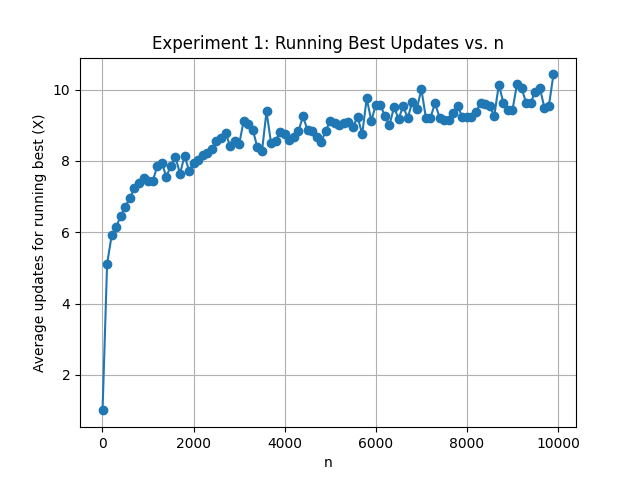
\includegraphics[width=0.45\textwidth]{E1_10k.png}} & \subfloat[100000 iterations with step of 1000]{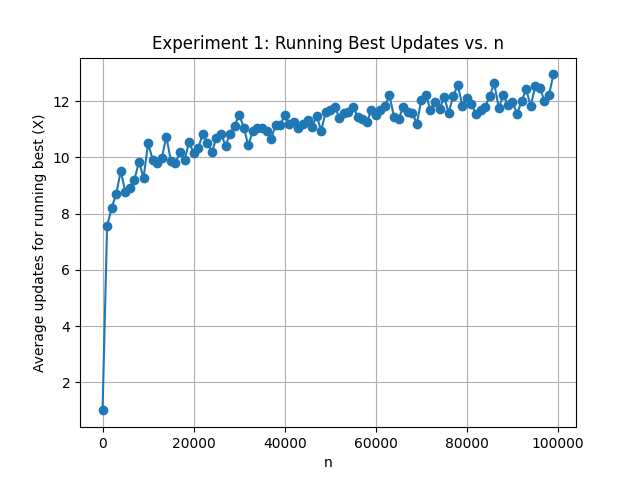
\includegraphics[width=0.45\textwidth]{E1_100k_1ksteps.png}} \\ \hline
        \end{tabular}
      \end{figure}
      From the above figures we can see that the average value of $X$ for increasing iterations follows a logarithmic trend empirically as well which gives weight to the theoretical claim that $X = O(\ln n)$.

      \textbf{Experiment 2} - Collisions in a Hash Table:
      \begin{figure}[H]
        \centering
        \begin{tabular}{|c|c|}
          \hline
          \subfloat[100000 iterations with step of 500]{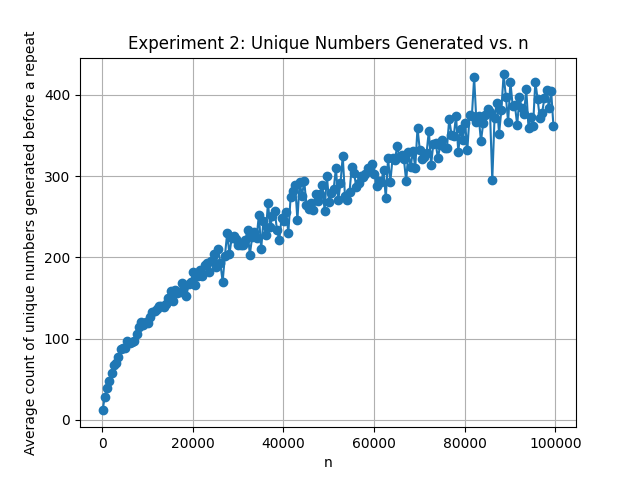
\includegraphics[width=0.45\textwidth]{E2_100k_500steps.png}} & \subfloat[100000 iterations with step of 1000]{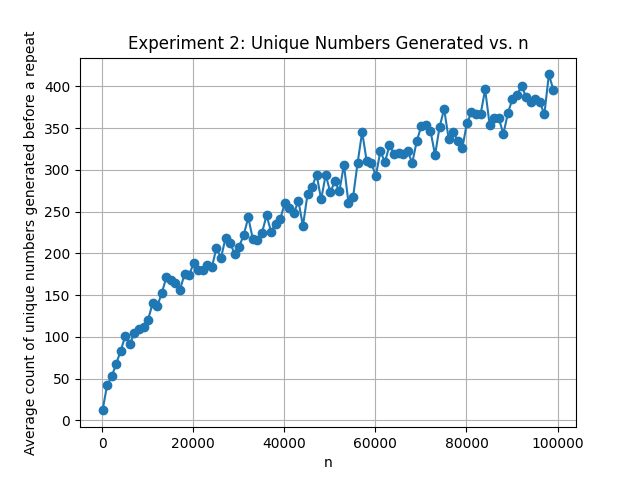
\includegraphics[width=0.45\textwidth]{E2_100k_1ksteps.png}} \\ \hline
        \end{tabular}
      \end{figure}

      From the above figures we can see that the average value of $X$ for increasing iterations follows a square root trend empirically as well which gives weight to the theoretical claim that $X = O(\sqrt{n})$.

      \textbf{Experiment 3} - Collecting Stickers:
      \begin{figure}[H]
        \centering
        \begin{tabular}{|c|c|}
          \hline
          \subfloat[10000 iterations with step of 500]{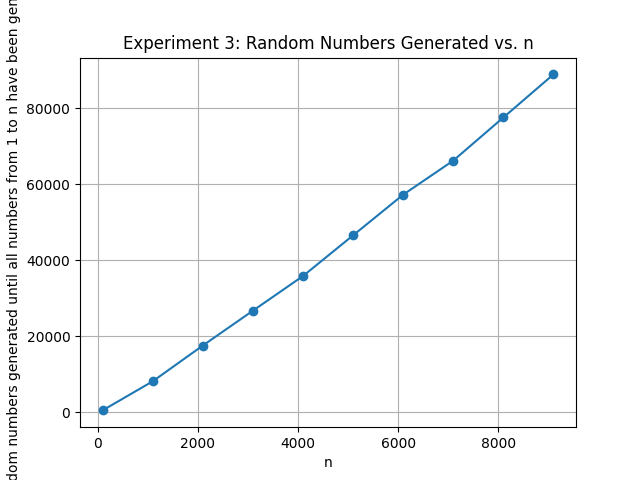
\includegraphics[width=0.45\textwidth]{E3_10k.png}} & \subfloat[100000 iterations with step of 1000]{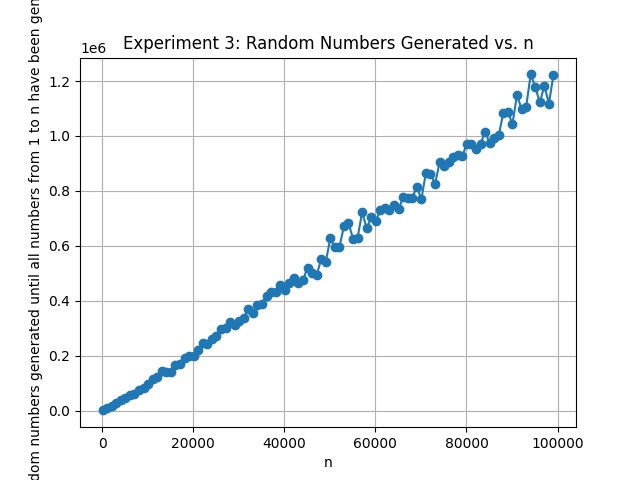
\includegraphics[width=0.45\textwidth]{E3_100k_1ksteps.png}} \\ \hline
        \end{tabular}
      \end{figure}

      From the above figures we can see that the average value of $X$ for increasing iterations follows a $n\ln n$ trend empirically as well which gives weight to the theoretical claim that $X = O(n\ln n)$.

\textbf{Code Listing that Generates the Above Plots:}
\begin{lstlisting}
import random
import matplotlib.pyplot as plt

def running_best_update(n): #Experiment 1
  sequence = list(range(1, n+1))
  random.shuffle(sequence)
  running_best = float('inf')
  updates = 0
  for num in sequence:
    if num < running_best:
      running_best = num
      updates += 1
  return updates

def urn(n): #Experiment 2
  unique_nums = set()
  count = 0
  while True:
    rand_num = random.randint(1, n)
    if rand_num in unique_nums:
      break
    unique_nums.add(rand_num)
    count += 1
  return count

def nuac(n): #Experiment 3
  nums_to_cover = set(range(1, n+1))
  nums_generated = set()
  count = 0
  while nums_to_cover:
    rand_num = random.randint(1, n)
    if rand_num in nums_to_cover:
      nums_to_cover.remove(rand_num)
    nums_generated.add(rand_num)
    count += 1
  return count

s = 100
e = 100001
step = 500

num_experiments = 100

def e1():
  n_values = []
  avg_updates = []

  for n in range(1, 100001, 1000):
    updates_sum = 0
    print(f"n: {n}")
    for _ in range(num_experiments):
      updates_sum += running_best_update(n)
    avg_updates.append(updates_sum / num_experiments)
    n_values.append(n)

  plt.plot(n_values, avg_updates, marker='o', linestyle='-')
  plt.xlabel('n')
  plt.ylabel('Average updates for running best (X)')
  plt.title('Experiment 1: Running Best Updates vs. n')
  plt.grid(True)
  plt.show()

def e2():
  n_values = []
  avg_counts = []

  for n in range(s, e, step):
    counts_sum = 0
    print(f"n: {n}")
    for _ in range(num_experiments):
      counts_sum += urn(n)
    avg_counts.append(counts_sum / num_experiments)
    n_values.append(n)

  plt.plot(n_values, avg_counts, marker='o', linestyle='-')
  plt.xlabel('n')
  plt.ylabel('Average count of unique numbers generated before a repeat')
  plt.title('Experiment 2: Unique Numbers Generated vs. n')
  plt.grid(True)
  plt.show()

def e3():
  n_values = []
  avg_counts = []

  for n in range(s, e, step):
    counts_sum = 0
    print(f"n: {n}")
    for _ in range(num_experiments):
      counts_sum += nuac(n)
    avg_counts.append(counts_sum / num_experiments)
    n_values.append(n)

  plt.plot(n_values, avg_counts, marker='o', linestyle='-')
  plt.xlabel('n')
  plt.ylabel('Average count of random numbers generated until all numbers from 1 to n have been generated at least once')
  plt.title('Experiment 3: Random Numbers Generated vs. n')
  plt.grid(True)
  plt.show()

e1()
e2()
e3()
\end{lstlisting}
    \end{solution}
\end{questions}
\end{document}